\documentclass[10pt, a4paper, twocolumn]{jarticle}
%\documentclass[10pt, a4paper, twocolumn, uplatex]{jsarticle}
\usepackage{proceeding_bachelor}
\usepackage{tabularx}
\usepackage{booktabs}
\usepackage{multirow}
\usepackage{cite}
\usepackage{amsmath, amssymb}
\usepackage{svg}

% Title info. ======================================
\title{不確実性適応型損失関数による \\
頑健な医用画像セグメンテーション}

%%%%% 著者 %%%%%
\author{廣池 友哉}

%%%% 学籍番号 %%%%
\studentid{M243422}

%%%% 所属 %%%%
\affiliation{広島大学 大学院先進理工系科学研究科 情報科学プログラム}

%%%% 年度を書き換える %%%%
\proceedingname{2025年度修士論文中間発表予稿}

%%%% 卒論発表の日付を書く %%%%
\date{2025/9/19}


\begin{document}
%%%%%%%%%%%%% Header and Title %%%%%%%%%%%%%
\maketitle


%%% Please write your body text from here %%
\section{はじめに}
医用画像セグメンテーションは,医用画像中の全てのピクセルに対し
物体のクラスのラベルを推定することで,正常組織または異常組織の領域を抽出するタスクである.
特に近年では,ポリープ\cite{ji2022video}や頭頸部がん(HNC)放射線治療における危険臓器\cite{maleki2020machine}などに用いられている.

医用画像セグメンテーションは,多様な症例に対して頑健に機能することが求められるが,
対象領域のサイズや形状が画像ごとに大きく異なるため,頑健な検出が困難であるという課題がある.
この課題に対処するために,損失関数を工夫する手法が提案されてきた.
例えば分類タスクで広く使われているCross-Entropy Loss\cite{long2015fully}と比較して,
Dice Index と呼ばれる類似度指標に基づいて定義されているDice Loss\cite{milletari2016v}は,
少数クラスの誤差も全体の平均損失に大きく寄与するため,クラス不均衡下でも検出性能を向上させる効果がある.
また、Dice Lossの多くの拡張手法も提案されており,CT画像\cite{zhu2019anatomynet, 9109297}や
MRI画像\cite{KATO2024107695}において高い性能が報告されている.
しかし,これらのアプローチでは検出難易度に関わらず誤差関数の形状が固定されており,
検出難易度が高い画像に対する学習が不十分になり,頑健な検出が困難であるという課題がある.

そこで本研究では,検出難易度を画像毎に算出したものを学習に取り入れ,
誤差関数の形状を動的に変化させる手法を提案する.
具体的には,画像毎に形状を変更できる誤差関数であるPolyDice-1 Lossを用いる.
学習中には一定epoch毎に推論フェーズを挿入し,Monte Carlo Dropout\cite{pmlr-v48-gal16}(以下,MC Dropout)により
各画像毎に複数枚の予測画像を得た後,ピクセル単位で不確実性指標を計算し,そこから画像全体の不確実性指標を集約したものを難易度指標として算出する.
この難易度指標をPolyDice-1 Lossの学習に取り入れることで,検出難易度を考慮した頑健な検出を実現することができる.

本研究の最終的な目的は,画像毎のセグメンテーションの難易度指標を学習に取り入れ,
誤差関数の形状を適応的に変化させることである.その実現に向けた最初のステップとして,
本稿ではピクセル単位の不確実性指標が学習が進むにつれてどのように推移するかを検証する.

\section{提案法}
図に提案法の概略図を示す.
提案法では,学習中に$M$(epoch)毎にMC Dropoutを用いて画像毎に$N$枚の推論を行うことで,各画像の不確実性を算出する.
この不確実性を難易度指標として扱ったものを,PolyDice-1 Lossの係数の動的な調整に利用することで,頑健な検出を実現する.
テスト時には,この適応的学習によって得られた最終的なモデルを用いて単一の予測を行う.

\subsection{PolyDice-1 Lossの説明}

\subsubsection{Polynomial Dice Lossの導出}
Dice Lossを拡張し多項式展開することを考える.
$W \times H$(pixel)の画像に対し,
予測画像を$\hat{\mathbf{y}} \in \mathbb R ^ {W \times H}$,
その画像に対する正解画像を$\mathbf{y} \in \mathbb R ^ {W \times H}$とし,
$\hat{\mathbf{y}}, \mathbf{y}$,の位置$i, j$における画素値をそれぞれ添字$i, j$を用いて$\hat{y}_{ij}, {y}_{ij}$と表現すると,Dice Lossは下記の式で示される.

\begin{equation}
  \mathcal{L}_{\text{Dice}}(\hat{\mathbf{y}}, \mathbf{y}) = 1 - \frac{2 \sum_{i=1}^{W} \sum_{j=1}^{H} \hat{y}_{ij} y_{ij}}{\sum_{i=1}^{W} \sum_{j=1}^{H}(\hat{y_{ij}} ^ 2 + y_{ij} ^ 2)}
\end{equation}

ここで予測画像$\hat{\mathbf{y}}$と正解画像$\mathbf{y}$をそれぞれ一次元のベクトル$\hat{\mathbf{y}} ^ {\prime}, {\mathbf{y}} ^ {\prime}$
に平坦化し,L2ノルム$\Vert \cdot \Vert$と内積$\langle \cdot, \cdot \rangle $を用いて
Dice Lossは次式のように表現することができる.
\begin{equation}
  \begin{aligned}
    \mathcal{L}_{\text{Dice}} &= 1 - \frac{2 \langle \hat{\mathbf{y}} ^ {\prime}, {\mathbf{y}} ^ {\prime} \rangle}{\Vert \hat{\mathbf{y}} ^ {\prime} \Vert ^ 2 + \Vert {\mathbf{y}} ^ {\prime} \Vert ^ 2} \\
    &= 1 - \frac{2 \Vert \hat{\mathbf{y}} ^ {\prime} \Vert \Vert {\mathbf{y}} ^ {\prime} \Vert}{\Vert \hat{\mathbf{y}} ^ {\prime} \Vert ^ 2 + \Vert {\mathbf{y}} ^ {\prime} \Vert ^ 2}
    \times \frac{\langle \hat{\mathbf{y}} ^ {\prime}, {\mathbf{y}} ^ {\prime} \rangle}{\Vert \hat{\mathbf{y}} ^ {\prime} \Vert \Vert {\mathbf{y}} ^ {\prime} \Vert}
  \end{aligned}
\end{equation}

この式において,$s = \frac{2 \langle \hat{\mathbf{y}} ^ {\prime}, {\mathbf{y}} ^ {\prime} \rangle}{\Vert \hat{\mathbf{y}} ^ {\prime} \Vert ^ 2 + \Vert {\mathbf{y}} ^ {\prime} \Vert ^ 2}$,
$\theta = \frac{\langle \hat{\mathbf{y}} ^ {\prime}, {\mathbf{y}} ^ {\prime} \rangle}{\Vert \hat{\mathbf{y}} ^ {\prime} \Vert \Vert {\mathbf{y}} ^ {\prime} \Vert}$とおくと,
$\mathcal{L}_{\text{Dice}} = 1 - s \cos{\theta}$となり,
Dice Lossは2つの成分,すなわちベクトル間の角度$\theta$に基づく方向成分(コサイン類似度)と,
ベクトルの大きさに基づくスケール成分$s$から構成されていることがわる.
両方のベクトルが単位ノルムである場合、スケール成分$s=1$となり,Dice Lossはコサイン類似度そのものと一致する\cite{KATO2024107695}.
ここで,$\theta$は予測ベクトルと正解ベクトルのなす角であり,予測と正解が大きく異ならない,
つまり$\theta \approx 0$と仮定し,$\cos{\theta}$を$\theta = 0$まわりでテイラー展開すると以下のように近似できる.
\begin{equation}
  \cos{\theta} = 1 - \frac{\theta ^ 2}{2!} + \frac{\theta ^ 4}{4!} - \cdots
\end{equation}

スケール成分$s$を一定と仮定し,この近似式をDice Lossに代入して整理すると,以下のようになる.

\begin{equation}
  \begin{aligned}
  \mathcal{L}_{\text{Dice}} &= 1 - s \left(1 + \frac{1}{2!} \theta ^ 2 - \frac{1}{4!} \theta ^ 4 + \cdots\right) \\
  &= (1 - s) + s \left[\sum_{k = 1}^{\infty} \frac{(-1) ^ {k - 1}}{(2k)!} \theta ^ {2k}\right]
\end{aligned}
\end{equation}

ここで,各テイラー項の係数$\alpha_k$を$\alpha_k = \frac{(-1)^{k-1}}{(2k)!}$とすると,
Dice Lossを多項式展開したPolynomial Dice Lossは以下のように表現できる.

\begin{equation}
  \mathcal{L}_{\text{PolyDice}} = (1 - s) + s \sum_{k = 1}^{\infty} \alpha_k \theta ^ {2k}
\end{equation}

この損失関数を計算するために、角度$\theta$は以下のようにコサインの逆関数を用いて算出される.
\begin{equation}
  \theta = \arccos{\left(\frac{\langle \hat{\mathbf{y}} ^ {\prime}, {\mathbf{y}} ^ {\prime} \rangle}{\Vert \hat{\mathbf{y}} ^ {\prime} \Vert \Vert {\mathbf{y}} ^ {\prime} \Vert}\right)}
\end{equation}

このようにして,Dice Lossを幾何学的に解釈したうえでテイラー展開を用いることでPolynomial Dice Lossが導かれる.


\subsubsection{PolyDice-1 Lossの導出}
PolyLoss\cite{leng2022polyloss}のアプローチに倣い,多項式の次数に基づいてPolynomial Dice Lossのバリエーションを検討する.
まず,テイラー展開で得られた無限級数を第$K$項までで打ち切ることで,以下のような損失関数を定義する:

\begin{equation}
  \mathcal{L}_{\text{PolyDice-K}} = \mathcal{L}_{\text{PolyDice}} + s \sum_{k=1}^{K} \varepsilon_k \theta^{2k}
\end{equation}

Lengら\cite{leng2022polyloss}は,多項式展開の最初の$K$項に対してパラメータ$\epsilon_i(i = 1, \cdots, K)$を用い,
高次の項を省略し,低次の項を強調する損失関数を提案した.
具体的には次のように定義される:

\begin{equation}
  \mathcal{L}_{\text{PolyDice-K}} = (1 - s) + s \sum_{k=1}^{K} (\alpha_k + \varepsilon_k) \theta^{2k}
\end{equation}
%
%
しかし,これらのハイパーパラメータ$\epsilon_i$を調整するのは難しく,
特に医用画像セグメンテーションでは交差検証による検証が用いられるため,このような複雑なチューニングは実用的ではない.
Leng ら\cite{leng2022polyloss}は,第$1$項($\theta ^ 2$)のみを調整するだけで十分な性能向上が得られることを示し,よりチューニングが容易なケース$K=1$の損失関数を提案している.
これに従い,以下のようにPolyDice-1 Lossを定義する.

\begin{equation}
  \mathcal{L}_{\text{PolyDice-1}} = (1 - s) + s(\alpha_1 + \epsilon_1) \theta^2
\end{equation}

\subsection{MC Dropoutによる複数回の推論}

前節で導入したPolyDice-1 Lossを用いて学習を行う際に,
一定epoch毎に推論フェーズを挿入し,MC Dropoutにより複数枚の予測画像を得る.
MC Dropoutは,ニューラルネットワークの一部のユニットを確率$p$でランダムに不活化するDropout処理を
学習時のみでなく推論時にも用いることで,予測を分布として計算する手法である.
出力を落とすノードを$N$回変えることで,出力される値は$N$回分の推論結果の分布として得られ,
この集合は近似的に予測事後分布の標本集合として解釈できる.
提案法では,学習段階でM(epoch)毎に推論フェーズを挿入してDropoutを確率$p$でMC Dropoutを$N$回実行することで,
各学習段階で$N$枚の複数の予測画像を得る.
またDropout層はモデルの最も深いエンコーダおよびデコーダに配置した.
浅い層と比較してより高次な特徴を抽出する深い層にDropoutを配置することで,
高次な意味的判断におけるモデルの確信度がより直接的に反映されることが期待される.

\section{セグメンテーションの難易度指標の算出}

\subsection{ピクセル単位の不確実性指標の計算}
前節で画像毎に得られた$N$枚の予測画像に対し,ピクセル単位で不確実性指標を計算する.
不確実性指標として,以下の3つを検討する.

\begin{itemize}
  \item (a)予測分散:確率予測値の統計的なばらつきを測る指標であり,以下の式で表される.
  \begin{equation}
    \text{Var}(\hat{y}_{ij}) = \frac{1}{N} \sum_{n=1}^{N} (\hat{y}_{ij}^{(n)} - \mu_{ij})^2
  \end{equation}
  ここで,$\hat{y}_{ij}^{(k)}$は$k$回目のMC Dropoutの推論における画素$(i, j)$の予測値であり,
  $\hat{\mu}_{ij} = \dfrac{1}{N} \sum_{k = 1}^{N} \hat{y}_{ij} ^ {(k)}$は$\{\hat{y}_{ij} ^ {(k)}\}_{i = 1} ^ {N}$の平均値である.
  予測分散は個々の予測値の平均からの散らばり具合を示し,予測が不安定であるほど大きな値をとる.
  \item (b)予測エントロピー:$N$回の予測を平均した後の最終的な予測値の不確実性を測る指標であり,以下の式で表される.
  \begin{equation}
    H(\hat{y}_{ij}) = - \mu_{ij} \log{\mu_{ij}} - (1 - \mu_{ij}) \log{(1 - \mu_{ij})}
  \end{equation}
  この値はデータに起因する不確実性とモデルの知識不足に起因する不確実性の両方が含まれ,
  値が高いほど最終的な予測が曖昧である状態を意味する.
  \item (c)相互情報量:予測エントロピーから期待エントロピーを差し引いたものであり,以下の式で表される.
  \begin{equation}
    I(\hat{y}_{ij}) = H(\bar{\hat{y}}_{ij}) - \frac{1}{N}\sum_{k=1}^{N} H(\hat{y}_{ij}^{(k)})
  \end{equation}
  この値は予測エントロピーから予測分散を差し引いたもので,モデルの知識不足に起因する不確実を示す指標,
  すなわち,MC Dropoutによる各推論結果の一貫性を示す.
\end{itemize}

上記の指標を分析することで,予測の不安定さやデータおよびモデルの不確実性を評価できる.

\subsection{画像全体の難易度指標の算出}
前節で得られたピクセル単位の不確実性を用いて,画像全体の難易度指標を算出する.
具体的には,画像全体の不確実性の○○を難易度指標として採用する.
○○を用いることで,画像全体の××を評価できると考えられる.

\newpage

\section{実験}
\subsection{実験条件}
提案法の有効性を検証するために,医用画像セグメンテーションデータを用いて実験を行った.
データセットは大腸ポリープのCVC-ClinicDB\cite{BERNAL201599}を用い,$5$-fold 交差検証に基づき訓練データと
テストデータに分割された.なお,訓練データのうち$10 \%$をランダムに抽出し,検証データとした.
各画像は$W = 224$ pixel, $H = 224$ pixelでリサイズを行い,
過学習抑制のため,訓練データに対する空間的データ拡張として
$50\%$の確率で上下左右反転及び画像の明るさ・コントラストの変更を施した.

セグメンテーションモデルは$3$層のU-Net\cite{ronneberger2015u}を用い,
学習には,バッチサイズ$32$, 学習率$10 ^ {-3}$ のAdaptive moment
estimation(以下, Adam)\cite{kingma2014adam}を用いた.
最大エポック数は$200$に設定し,検証データに対する損失が最小のエポックにおける
モデルインスタンスを,最終的なテストデータの評価に用いた.

また,提案法におけるMC Dropoutのパラメータとして,
Dropoutを行う確率$p = 0.5$,推論回数$N = 10$,推論フェーズの挿入間隔$M = 10$とした.

\subsection{結果と考察}
学習初期に高い精度で予測できるようになった症例(以下症例$1$)と,学習後期においても精度が低い症例(以下症例$2$)について,
$50, 100, 150, 200$ epochのピクセル単位の不確実性指標の推移を示す.
(a)は予測平均,(b)は予測分散,(c)は予測エントロピー,(d)は相互情報量である.
なお各不確実性指標において,画像を表示する際の最大値および最小値は,2つの症例間から算出した.

図\ref{fold5_file144}に症例$1$の不確実性指標の推移を示す.
図\ref{fold5_file144}(b),(d)から,学習の進行に伴いポリープ内外で減少していることがわかる.
これはポリープ内外において,モデルが学習の初期に予測の安定性と内部的な一貫性を獲得し,
モデル自身の不確実性が解決された状態を示している.
一方,両指標ともにポリープの境界部分では,学習後期においても微小な不確実性が残存している.
これはモデル自身の不確かさが解消された後も残る不確実性,すなわちデータ自体が持つ本質的な曖昧さを反映していると考えられる.

図\ref{fold2_file450}に症例2の不確実性指標の推移を示す.
図\ref{fold2_file450}(b),(d)から,症例$1$と異なり,学習の進行に伴い,
ポリープの輪郭および内部において不確実性が増大していることがわかる.
これは症例$1$とは対照的に,モデルの内部的な予測確率の違いが最後まで解消されず,予測が数値的にも安定していないことを示している.
症例$2$のポリープは,他の組織の特徴と類似しているため,
モデルが学習データから一貫した判断基準を確立できなかったことが原因で最後まで精度が低かったと考えられる.
すなわち,学習に伴い不確実性が増大しているのは,モデル自身の知識不足を反映していると考えられる.

上記のピクセル単位の不確実性指標として,
不確実性指標は境界領域に集中する傾向が見られたため,集約方法として,
画像全体の平均値ではなく,境界領域に限定して集約した指標を用いることで,
よりセグメンテーション性能に直結した難易度指標を定義することができると考えられる.
また症例2において,学習の進行に伴い不確実性が増大したことから
学習の後半で難易度指標が増大している症例に関しては,$\epsilon_1$の値を増加させ,
誤った予測を行った画像の組織の特徴を重点的に学習させるような損失関数を設計することで
頑健な検出を行うことができると考えられる.


\section{まとめと今後の課題}
本稿では,医用画像セグメンテーションの誤差関数において,検出難易度が高い画像に対する学習が不十分になり,頑健な検出が困難であるという課題に対処するため,
検出難易度を画像毎に算出したものを学習に取り入れ,誤差関数の形状を動的に変化させる手法を提案した.
提案法では,学習中に一定epoch毎に推論フェーズを挿入し,MC Dropoutにより複数枚の予測画像を得た後,
ピクセル単位で不確実性指標を計算した.
医用画像セグメンテーションデータを用いた実験の結果,学習後期においても精度が低い症例に関して,
ピクセル単位の相互情報量の分散と相互情報量が増大していくことが明らかになった.
今後は,上記の不確実性指標を領域周辺に着目して集約する方法を検討し,
難易度指標が高い症例の特徴を重点的に学習できる損失関数を設計することで,提案法の有効性を検証する予定である.

\newpage

\begin{figure*}[t] % ← [t]をここに移動する
  \begin{center}
    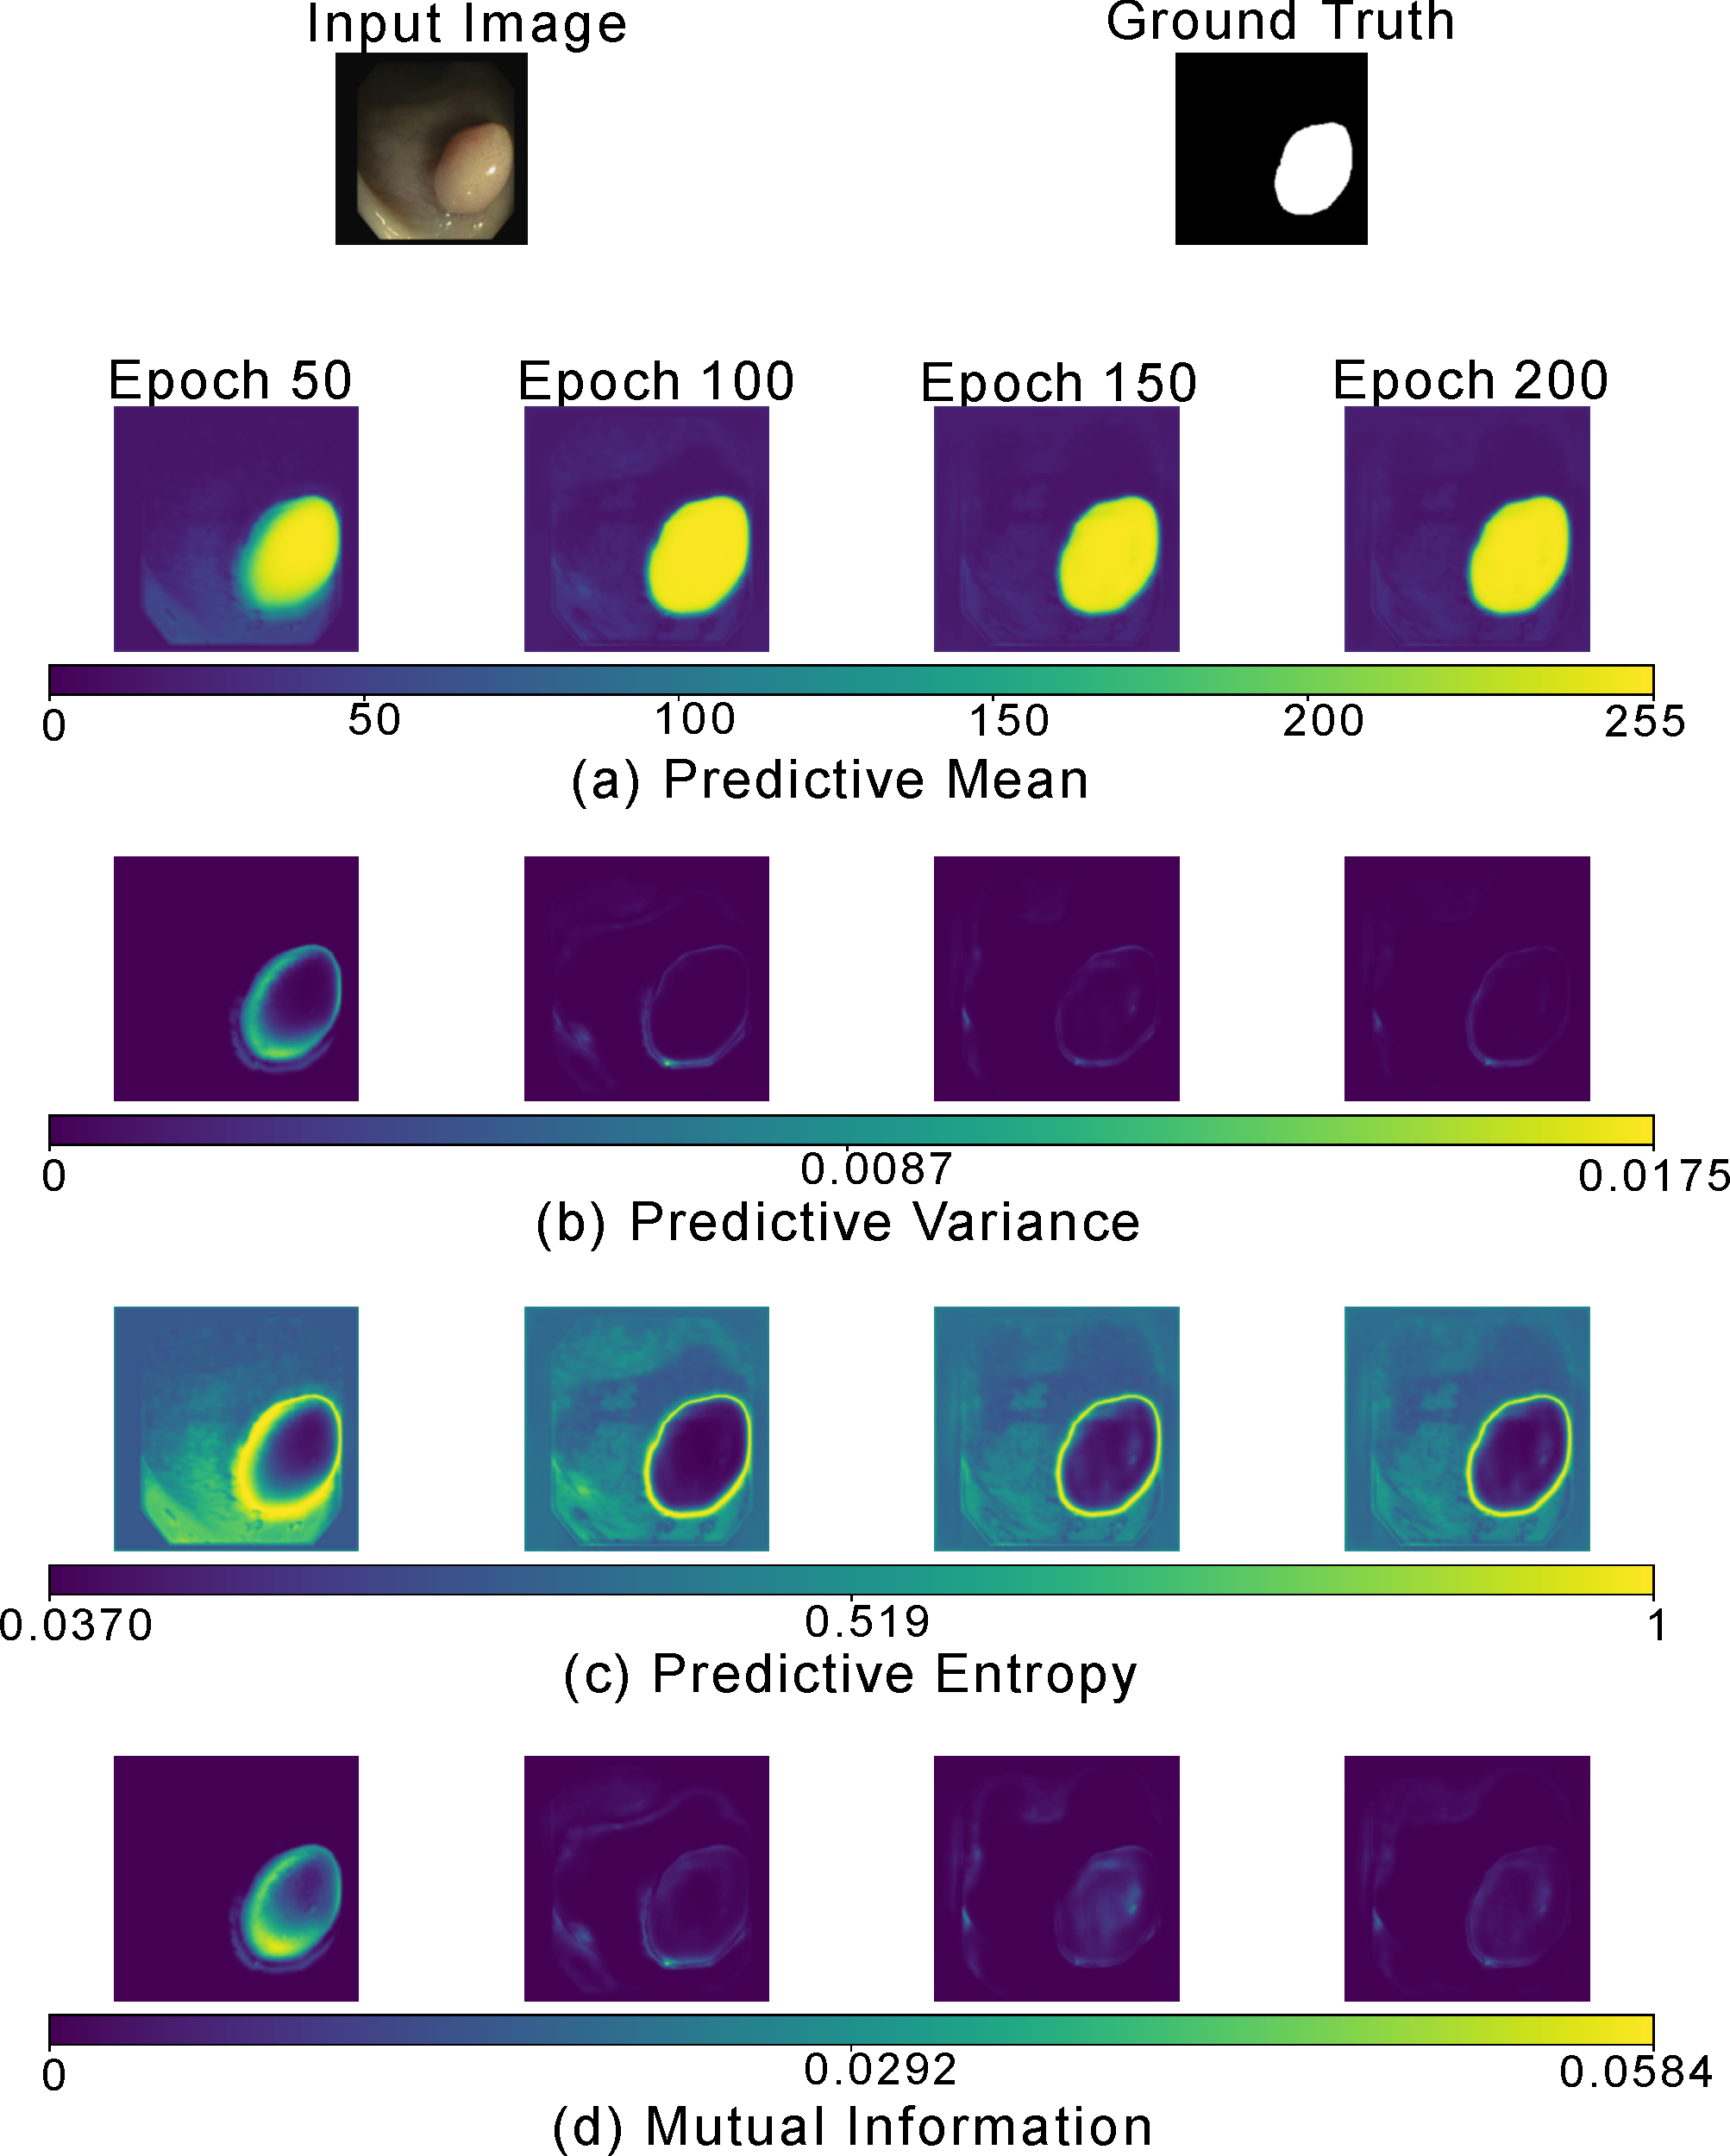
\includegraphics[scale=0.25]{figure/fold5_file144_uncertainty_evolution.pdf}
    \caption{Example of Cases that are learned quickly with high accuracy:
    (a) Predictive Mean, (b) Predictive Variance,
    (c) Predictive Entropy(d) Mutual Information}
    \label{fold5_file144}
  \end{center}
\end{figure*}

\begin{figure*}[t] % ← [t]をここに移動する
  \begin{center}
    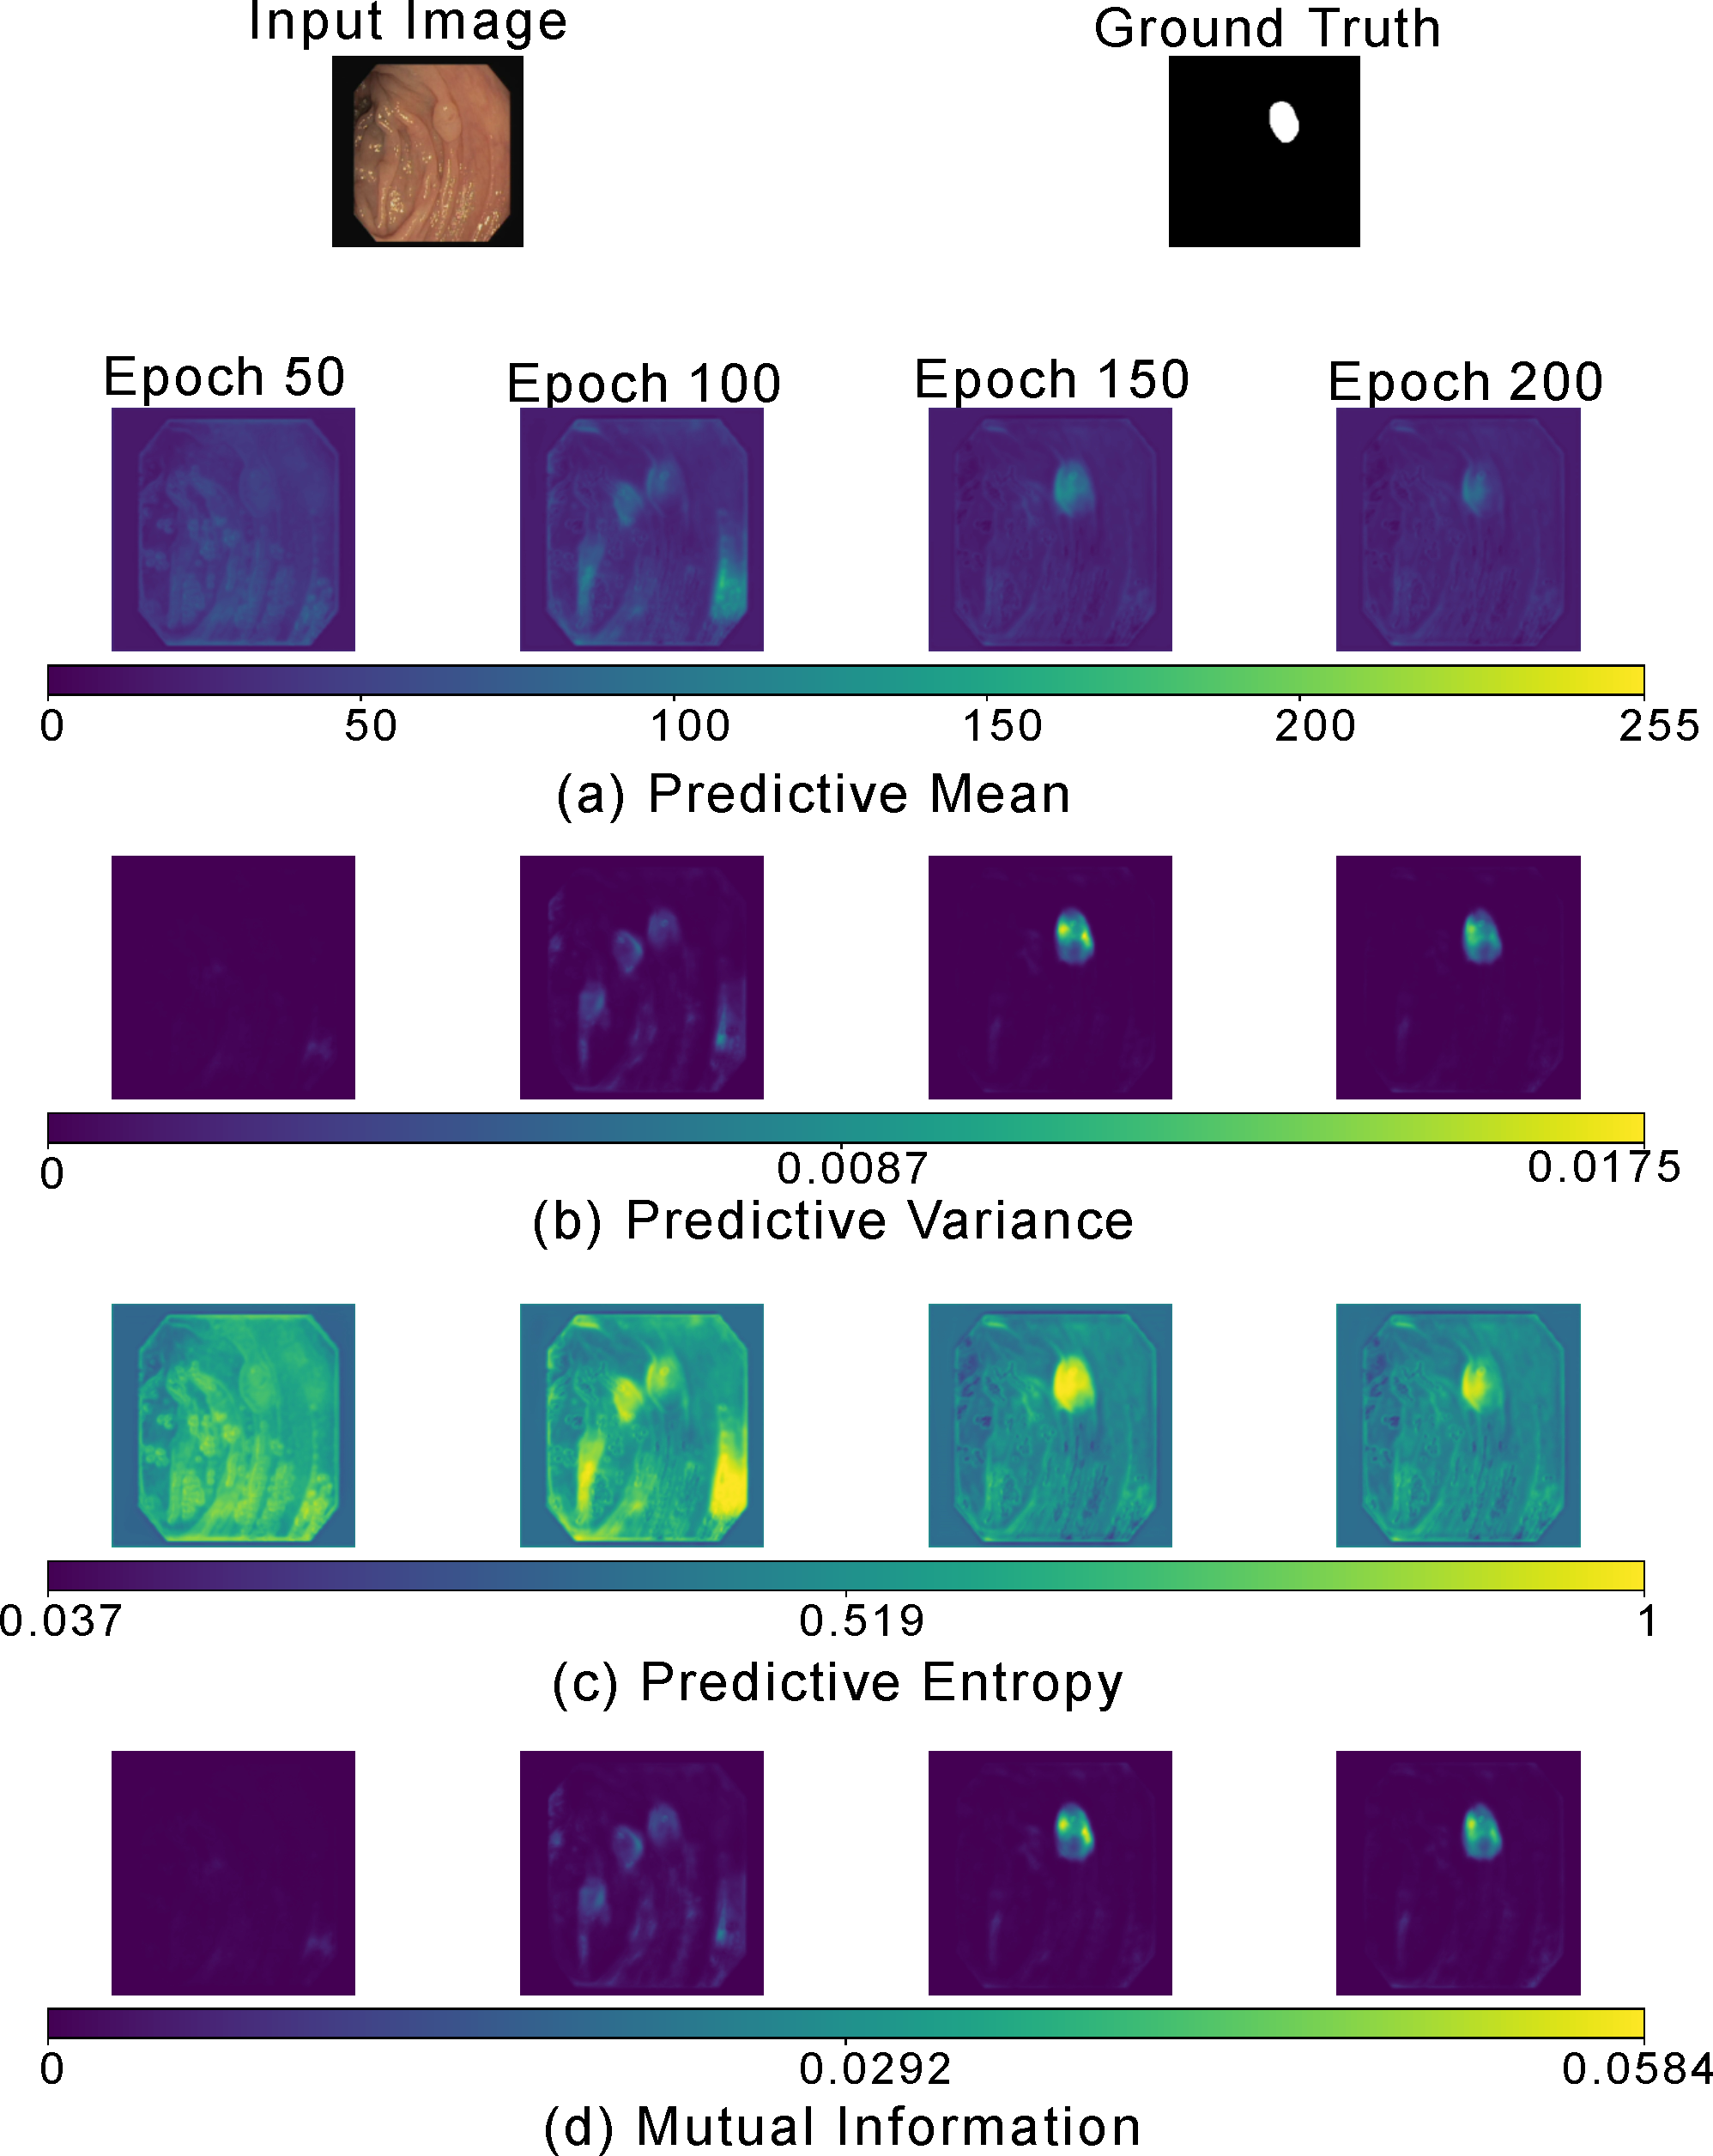
\includegraphics[scale=0.25]{figure/fold2_file450_uncertainty_evolution.pdf}
    \caption{Example of Challenging cases with persistently low performance:
    (a) Predictive Mean, (b) Predictive Variance,
    (c) Predictive Entropy(d) Mutual Information}
    \label{fold2_file450}
  \end{center}
\end{figure*}

\clearpage

%%%%% 参考文献(BibTeXを使う場合) %%%%%
\bibliographystyle{bibstyle} % bstファイルを設定
\bibliography{references} % bibファイルを読み込み

%%%%% 参考文献(直接書く場合) %%%%%
% \begin{thebibliography}{9} %\footnotesize
    % \bibitem{kajiya1986rendering}
    % J.~T. Kajiya,
    % \newblock ``The rendering equation,''
    % \newblock in {\em Proceedings of the 13th Annual Conference on Computer
    %   Graphics and Interactive Techniques}, pp. 143--150, 1986.
    
    % \bibitem{jensen2001realistic}
    % H.~W. Jensen,
    % \newblock {\em Realistic image synthesis using photon mapping}, vol. 364,
    % \newblock Ak Peters Natick, 2001.
% \end{thebibliography}

\end{document}